\documentclass[english]{article}

\usepackage{babel}
\usepackage{graphicx}
\usepackage{times}
\usepackage{pifont}
\usepackage[margin=1in]{geometry}
\usepackage{eurosym}
\usepackage{fancyhdr}
\usepackage[hidelinks]{hyperref}
\usepackage{float}

\pagestyle{fancy}
\fancyhf{}


%HEADER
%**************************************************************************************
\pagestyle{fancy}
\fancyhf{}
%**************************************************************************************
\lhead{Internship Report}		 	 
\rhead{Savonia University of Applied Sciences} 
\lfoot{EFA12SF}
\cfoot{\thepage}
\rfoot{Alexey Tukalo}
%**************************************************************************************

\date{}
\setlength\parindent{0pt}

\begin{document}

\title{\vspace{2in}INTERNSHIP REPORT\\
\small Savonia University of Applied Sciences\\
\vspace{0.5in}
\includegraphics{savonia.jpg}}

\nopagebreak
\maketitle


\vspace{3in}

\author{
\begin{flushleft}
Student name: Alexey Tukalo,\\
Student number: 67687,\\
Group: EFA12SF,\\
Type: The internship information technologies,\\
Duration: 4 months and 1 week or 720 hour (07.07.2015-18.11.2015)\\
The day of the report: \date{\today}
\end{flushleft}
}

\thispagestyle{empty}

\newpage
\setcounter{page}{1}
\setcounter{tocdepth}{2}
\tableofcontents

\newpage

%MAIN CONTENT ******************************************************************************************************************

\section{Company}

I carried out my summer practice at Institute of Data Processing and Electronics, which belonges to the Karlsruhe Institute of Technology (KIT). The organisation's visitor address is Hermann-von-Helmholtz-Platz 1, 76344 Eggenstein-Leopoldshafen, Germany and mailing address is Karlsruhe Institute of Technology (KIT) - Campus North, Institute for Data Processing and Electronics (IPE), P.O. Box 3640, 76021, Karlsruhe, Germany. The phone number is +49 721 608 2 2027, an e-mail address is info@ipe.kit.edu, ipe.kit.edu is the webpage of the organisation. I worked under supervision of Dr. Torsten Hopp. His e-mail address is torsten.hopp@kit.edu and the phone number is +49 721 608-25990. The internship period was from the 7th of July to the 18th of November.

\subsection{General Information}

Karlsruhe Institute of Technology is one of the largest research and education organisations in Germany. In 2009, University of Karlsruhe merged with Research Center Forschungszentrum Karlsruhe\footnote{Based on national nuclear research center opened in 1956 and called Kernforschungszentrum Karlsruhe, or KfK}. The institute has leadership in the Engineering and Natural Sciences in Europe, ranking sixth overall in citation impact.\\

The total budget of KIT is \euro 844 million, the total number of stuff is over 10 000 and over 7000 of them is academic stuff. There are 24500 students, 12600 of them are undergraduates ones, 8300 are postgraduate and over 800 are doctoral students.
\subsection{Stuff}

I was a part of the 3D Ultrasound Computer Tomography (USCT) team. USCT and the Big Data research group together form the Software Methods group of IPE. The Head of the Software Methods group is Dr. Rainer Stotzka. The permanent part of USCT team consists of:

\begin{itemize}
\item Dr. Nicole Ruiter - the head of 3D USCT
\item Dr. Torsten Hopp - responsable for image processing and data management
\item Michael Zapf - responsable for hardware and software integration
\item Prof. Dr. Hartmut Gemmeke - former head of IPE, now advisor of 3D USCT
\end{itemize}

Other team members are students who are doing internship or these at the institute.

\section{History}

\subsection{KIT History}

A polytechnic school of Karlsruhe was founded on the 7th of October 1825. In 1865, the schooles was raised to the status of an institution of higher education. Since 1885 the organisation was called institute of technology. In 1967, it started to be called University. Karlsruhe Nuclear Research Centre was opened in 1956. \\

University of Karlsruhe opened a central computer laboratory and became one of the leading German institutions in computer science, in 1986. Karlsruhe Research Centre and Karlsruhe Institute of Technology merged together at 1 October 2009.

\subsection{IPE History}

IPE was founded as a part of Institute for Neutron Physics and Reactor Technology in 1959. It evolved to the Centre of Data Processing Department Laboratory Automation in 1967-1971. In 1973, the Computing Centre Data Processing and Laboratory for Electronics and Measurement Instrumentation merged in Department for Data Processing and Instrumentation. In 1991, the Department Data Processing and Electronics became independent from the Department for Data Processing and Instrumentation. Since 2001, the organisation is called Institute for Data Processing and Electronics.

\section{Work description}
\subsection{Project description}
\begin{figure}
\centerline{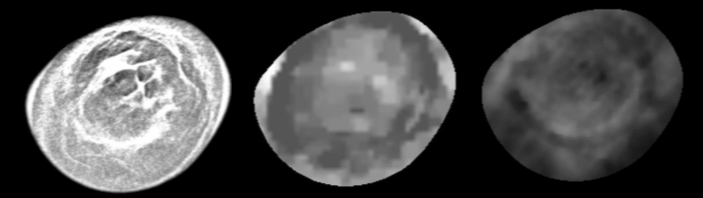
\includegraphics[scale=0.5]{internship_report/images.png}}
\caption{Examples of reflection, sound speed, attenuation images\label{fig:example}}
\end{figure}
I worked in a project called 3D Ultrasound Computer Tomography, shortly USCT. The main goal of the project is to develop a new imaging methodology for early breast cancer detection. This type of cancer is one of the most common and dangerous ones among women. A breast is not a vital organ, so the majority of patient dies of metastasis. A tumor with a size less than 5mm has very low probability of metastasis.  That's why, an early diagnosis of breast cancer significantly increases the survival probability of the patient. The USCT team's aim is detection of the tumor with an average size smaller than 5mm. 

The USCT system is able to produce three different types of images (Pic. \ref{fig:example}):

\begin{enumerate}
\item Reflection - contains general structure by imaging tissue surfaces
\item Sound speed - map of the sound speed distribution
\item Attenuation - map of the sound wave's amplitude attenuation
\end{enumerate}

The sound speed and attenuation images give doctors an opportunity to classify lesions precisely  (Figure \ref{fig:nicol}), while the reflection one allows them to define the structure. An essential part of the image processing is to fuse the three different images into a single one in order to give an intuitive access to the multimodal information at a glance and it was my main task of my internship. 

\begin{figure}[H]
\centerline{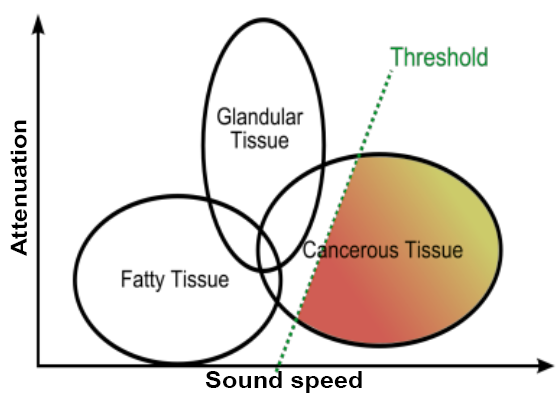
\includegraphics[scale=0.5]{internship_report/nicol}}
\caption{Tumor clasification based on sound speed and attenuation\label{fig:nicol} \cite{nicol}}
\end{figure}
\subsection{Position description}

3D USCT volumes are converted into stacks of 2D images along specified standard slicing directions used in radiological workflows. They are presented to radiologist using USCT's customized edition of DICOM Viewer, which is based on the ImageJ Framework and the Tudor DICOM Viewer. The aim of my internship was to explore new intuitive ways of multimodal data visualization, create the prototype of the methods and implements the visualizations in the customized DICOM Viewer. The software should be extended accordingly to allow interactive access to the visualization, e.g. to allow user specified input for setting thresholds, choosing projection directions etc.\cite{p}\\

I also have had my personal goals related with the internship:
\begin{itemize}
\item Improve skills on object-oriented programming with Java\footnote{Java is one of the main languages studied in my program at Savonia UAS} and improve knowledge of MATLAB
\item Gain an experience in digital image processing
\item Get an experience in team work on real-life project
\item Learn software development workflow
\end{itemize}
I did not have any experience in digital image processing before the internship, but I have had deep understanding of color theory, visual art and raster graphics, which helped me a lot.

\subsection{Work description}
\subsubsection{Prototyping}

The most part of my internship I worked on development of new fusion techniques for 3D USCT images under supervision of Dr. Hopp. During the first week I made a literature research and came up with several ideas for realization of the fusion. After that I created prototypes for three promising approaches in MATLAB. The picture \ref{fig:prot} demonstrates prototype of HSV Fusion, which was chosen as the best solution.\\

\begin{figure}
\centerline{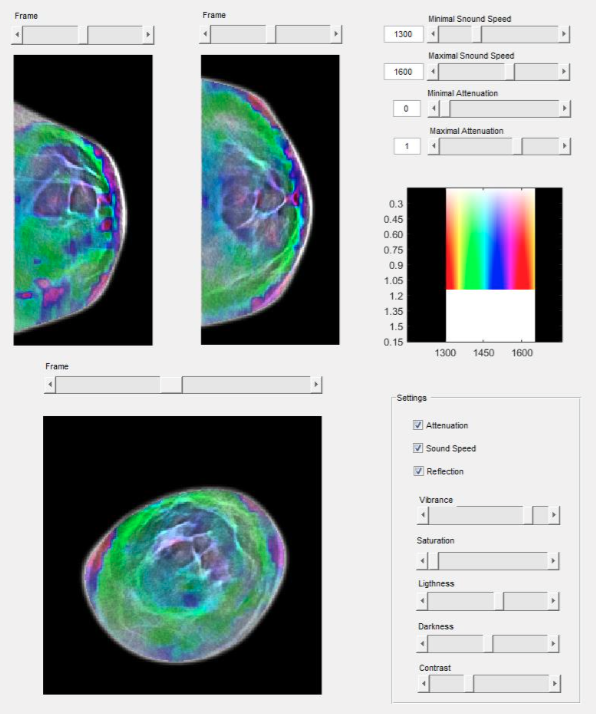
\includegraphics[scale=0.4]{internship_report/pro}}
\caption{MATLAB prototype for HSV Fusion\label{fig:pro}}
\end{figure}
\subsubsection{HSV Fusion}

The algorithm is based on the HSV color model. The model divides the color of every pixel into three separate components:

\begin{itemize}
\item Hue - keeps chromatic information (if the pixel is red, green, blue etc.)
\item Value - keeps grayscale information (how bright is the pixel)
\item Saturation - keeps an information about saturation of the hue (how far away is the color from gray)
\end{itemize}

\begin{figure}[H]
\centerline{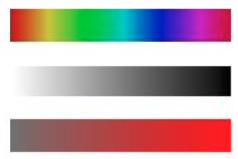
\includegraphics[scale=0.6]{internship_report/hsv}}
\caption{Components of HSV image from top to bottom: Hue, Value, Saturation.\label{fig:hsv}}
\end{figure}

The components are shown in figure \ref{fig:hsv}. The color space of the model can be represented as cylinder, where: altitude is the value, saturation is radius from the center and the angle is hue, see figure \ref{fig:model}.\\

To get the final result of the fusions. The algorithm transfers the image from HSV to RGB color model. The visual representation of the conversion is shown in figure \ref{fig:hsv2rgb}. The picture is very easy to read because the data is separated over three different domain natural for human vision.\\

\begin{figure}[H]
\centerline{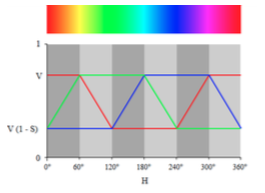
\includegraphics[scale=0.7]{internship_report/hsv2rgb}}
\caption{Visuale representation of HSV to RGB convertions\label{fig:hsv2rgb}}
\end{figure}

\subsubsection{DICOM Viewer realisation}

The prototype was presented to the Software Methods groupe of IPE. The realisation got positive feedback from the team and I started the realization of the algorithm in DICOM Viewer with ImageJ.\\


The DICOM realisation has a simpler user interface than the MATLAB implementation, to make it better understandable for an end user. Sound speed thresholding were added to the final version of fusion, figure \ref{fig:final}.

\begin{figure}
\centerline{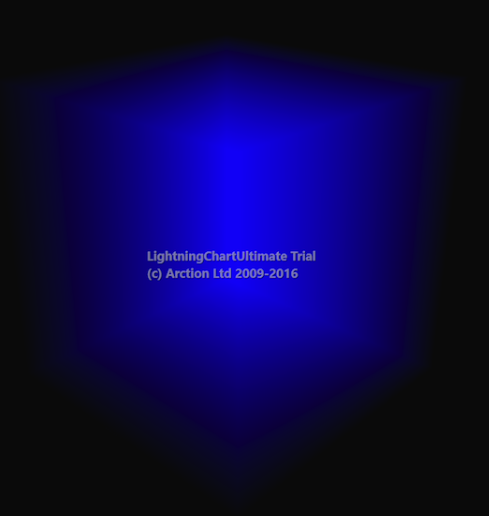
\includegraphics[scale=0.5]{internship_report/final}}
\caption{DICOM Viewer HSV Fusion Menu \label{fig:final}}
\end{figure}

\subsubsection{Re-slicing}

DICOM Viewer kept three seperate stacks of images for the different slicing directions along the x, y and z axis. Yet, thereby the same information needs to be stored three times as every of this three stacks contains enough information for visualising of all three slicing directions.\\
\begin{figure}[H]
\centerline{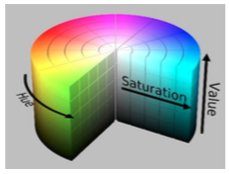
\includegraphics[scale=0.7]{internship_report/model}}
\caption{Model of HSV color space\label{fig:model}}
\end{figure}
My task was to implement the slicing algorithm, which allows to recalculate all three slicing directions from any of them directly within the DICOM viewer. If the image resolution along different axis is not uniform the algorithm also had to perform interpolation of the data.\\

Re-slicing is very useful feature for DICOM Viewer, because it will three times reduce the size of the image database by a factor of three and it will give an opportunity to also browse different slice directions of MRI images, which are usually used for comparison with USCT images in the same DICOM Viewer.\\

\subsubsection{WebGL Visualisation for USCT}

I was volunteer to take part at development of 3D WebGL Visualisation of USCT data and Dr. Hopp allowed me to join the team. Michael Zapf was responsable for development of the project and the last part of my internship I did under his control.\\

The vizualisation is based on Tomoraycaster 2\footnote{JavaScript framework for visualisation of 3D data, developed in IPE}. The aim was to modify the framework to make it works with USCT data well and develop a sci-fi graphical user interface for better representation of the visualisation.\\

My work started with deployment of an example for Tomoraycaser 2 with USCT data. The example was able to show the breast structure from reflection image. After that I started to make an adoptatoin of the shaders to give them an opportunity to handle multimodal data. This allowed me to integrate the image fusion, but I also added severl other features to the realisation. The visulisation was quite slow on weak machines when I started my developments. That's why I also worked on optimization of the code.\\

\begin{figure}[H]
\centerline{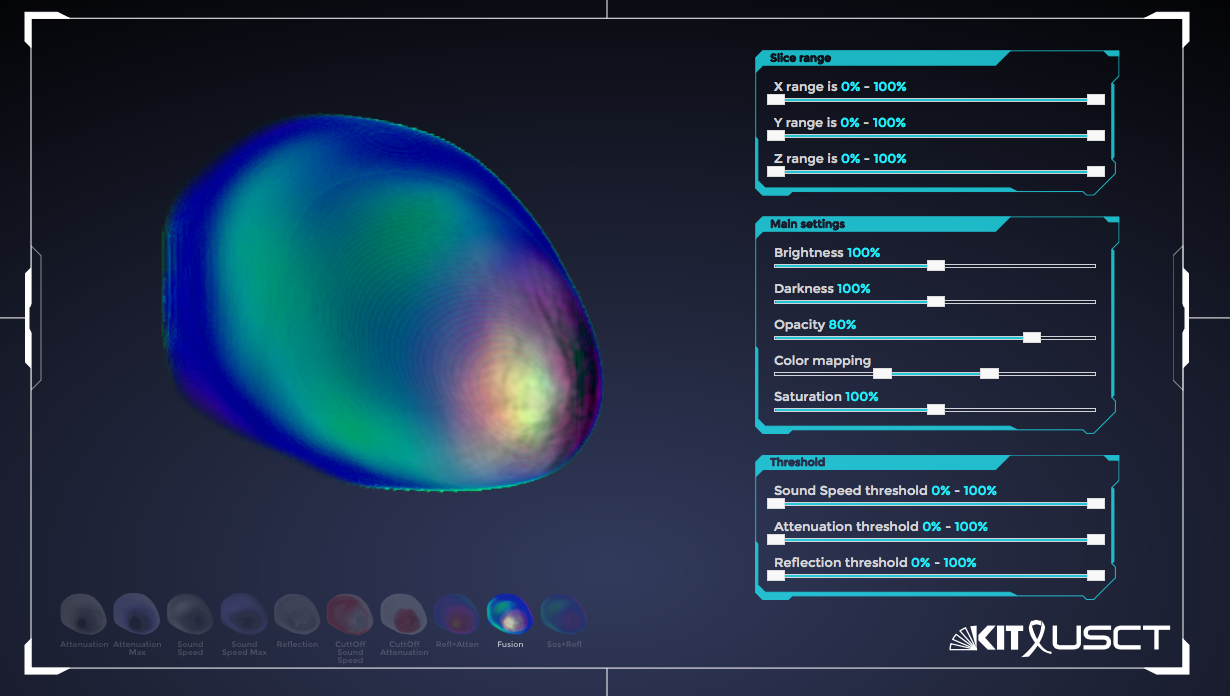
\includegraphics[scale=0.4]{internship_report/usct}}
\caption{Web visualization for 3D USCT\label{fig:usct}}
\end{figure}

When I finished my modifications for Tomoraycaster, I started to write the actual graphical user interface in according with skeleton of the project provided to me by Nicolas.\\

Our GUI has a very complex animation and designe. That's why I decided to draw the entire website inside a dynamic SVG image. I used Snap.SVG library to draw SVG images dynamically inside the webpage. Tomoraycaster and jQuer UI sliders were added to the SVG image as foreign objects.\\

The final result of the work is a 3D visualization of the USCT data with ten different modes and eleven sliders with different parameters, see pic. \ref{fig:usct}. The visualization is available at http://ipepc57.ipe.kit.edu:10002

\subsection{Working place communication}
During the most part of my internship I worked under direct supervision of Dr. Torsten Hopp. I received the task from my supervisor, asked him for help when I have had problems and reported about the current progress. My work on the modifications of the DICOM Viewer was organised via SVN version control system, so I worked in my own branch to prevent any additional bugs in the main repository. Dr. Hopp was always able to get my latest stable result, to check the code style and report about bugs. Every new feature implemented in DICOM Viewer was checked by Dr. Hopp and fixed by me in according with his feedback. Finally my branch was merged with the main repository.\\

Every Wednesday the USCT group had a meeting. The meeting starts with a discussion about current news related to the project. After that we have had a so called "weekly round", during which every team member reported about his/her progress during the last week in front of USCT team. During the report everyone was able to request help or advise from others or help somebody him/herself. \\

At the last part of my internship I worked in cooperation with Nicolas Tan. He is an experienced web developer responsible for development and maintenance of Tomoraycaster 2. Therefore he was assigned as my mentor for the task. I was very happy to have an opportunity to work under his mentoring, because it was perfect chance to improve my knowledge in the field of web development.\\

During the development of the visualization I worked in close cooperation with my mentor. We had discussions about the key issues of the project and made the key decisions together. He checked my code and tought me a lot about using Git as versioning system and writing a good code. The requirements for the project were developed and controlled by Michael Zapf. Sometimes three of us had a small meetings to make key discussions. Michael also visited my working place to check current progress, point to bugs and give some advises.

\section{Conclusion}

I was very satisfied with the internship because I reached my personal goals and in my point of view the task assigned to me was sorted well. In accordance with the postion goals during the internship I developed a new way of visualizing for multimodal USCT data. During the implementation of the prototype for the algorithm in MATLAB, I improved my knowledge of MATLAB. After that I gained an experience in object-oriented programming with Java and digital image processing, during integration of the algorithm in DICOM Viewer and development of the reslicing. I also learned in practise the software development workflow from idea, to prototype and from prototype to implementation and testing.\\

During the second part of my internship I got an experience in team work on real-life project, I improved my knowledge of tools for team cooperation such as the Git version control system. I also studied in practice the web development workflow and web development tools like browserify and sass, improved my system administration skills during deployment of the application. Nicolas' guidance helped me to improve my coding style and made my understanding of JavaScript much deeper.\\

I am very thankful to KIT for this experience, because I want to build my career in the field of digital image processing, visualization and computer graphics. The work placement gave me first industrial experience in this fields, so it means a lot for my future career prospects.\\

I am very thankful to all the people I met during the internship, to the Software Methods group of IPE and especially to Dr. Hopp, Nicolas Tan and Michael Zapf for the mentoring and knowledge provided by them.

\newpage
\begin{thebibliography}{1}

   \bibitem{nicol} USCT Presentation by Dr. Nicole Ruiter
   
   \bibitem{p} Position proposal from Dr. Torsten Hopp

\end{thebibliography}


\end{document}
